\section{Туршилт ба дүрслэл}
\subsection{Safety шалгалтыг гараар давтах нь}
Алгоритм «яг одоо ямар процесс дуусаж чадах вэ?» гэсэн асуултаар эхэлнэ. \textit{Work} нь шалгалтын явцад сул гэж тооцох нөөцийн түр хуулбар бөгөөд эхний утга нь Available. Дуусаагүй процессын Need векторын бүх элемент Work-ийн харгалзах элементээс ихгүй бол уг процесс ажлаа дуусгаж чадна. Тэр процессын одоо эзэмшиж байгаа Allocation-ийг Work-д нэмж, дараагийн процессыг сонгоно.

Жишээний эхэнд P0-д R0-оос 7 хэрэгтэй ч Work-д 3 байна. P1-д шаардлагатай $(1,2,2)$ нь $(3,3,2)$-т багтана. P1-ийг дууссан гэж үзвэл анх эзэмшиж байсан $(2,0,0)$ чөлөөлөгдөж Work $(5,3,2)$ болно. Цөм процессын дугаарыг багаас их рүү шалгаж, дуусгаж болох эхний процессыг сонгодог.

\tbl{Safety шалгалтын таван алхам}{tab:safety}{
\begin{tabularx}{\linewidth}{c c CCCC}\toprule
\hd № & \textbf{Процесс} & \textbf{Work өмнө} & \textbf{Need} & \textbf{Чөлөөлөх} & \textbf{Work дараа}\\\midrule
1 & P1 & $(3,3,2)$ & $(1,2,2)$ & $(2,0,0)$ & $(5,3,2)$\\
2 & P3 & $(5,3,2)$ & $(0,1,1)$ & $(2,1,1)$ & $(7,4,3)$\\
3 & P0 & $(7,4,3)$ & $(7,4,3)$ & $(0,1,0)$ & $(7,5,3)$\\
4 & P2 & $(7,5,3)$ & $(6,0,0)$ & $(3,0,2)$ & $(10,5,5)$\\
5 & P4 & $(10,5,5)$ & $(4,3,1)$ & $(0,0,2)$ & $(10,5,7)$\\\bottomrule
\end{tabularx}}

Гурав дахь мөрөнд P0-ийн хэрэгцээ Work-тэй яг тэнцүү тул процесс дуусаж болно. Тав дахь мөрийн дараа Work нь системийн нийт нөөц $(10,5,7)$-той тэнцсэн. Иймээс P1 → P3 → P0 → P2 → P4 нь аюулгүй дараалал мөн. Бүх процессыг багтаасан нэг дараалал олоход SAFE дүгнэлт хийхэд хангалттай.

\lead{Яагаад Work-д зөвхөн Allocation нэмдэг вэ?} Тухайн процесс үлдсэн Need-ээ Work-оос аваад ажлаа дуусмагц өмнөх Allocation болон шинээр авсан Need хоёуланг буцаана. Work-ийн цэвэр өсөлт нь өмнө эзэмшиж байсан Allocation-тэй тэнцэнэ. Энэ тооцоо зөвхөн боломжит дарааллыг шалгадаг тул графын «Дараах» товчийг дарахад серверийн бодит Available өөрчлөгдөхгүй.
\lead{Дарааллыг хөтчөөр тулгах нь.} Номын жишээн дээр тоглуулагчийг эхэнд нь байрлуулна. Эхний алхмын өмнө Work $(3,3,2)$, дууссан процессын тоо 0 байна. Нэг алхам ахихад P1-ийн эзэмшиж буй R0-ийн хоёр нэгж чөлөөлөгдөж Work-ийн эхний тоо 3-аас 5 болно. Хоёр дахь алхамд P3 нь R0, R1, R2-оос харгалзан 2, 1, 1 нэгж буцаана. Дэлгэцэд $(7,4,3)$ гарвал граф, хүснэгт хоёул ижил тооцоог харуулж байна.
\newpage
\subsection{Нөөц хүсэх шийдвэрийн схем}
Хүсэлт ирэхэд цөм гурван асуултад дарааллаар нь хариулна. Зураг~\ref{fig:decision}-ийг дээрээс доош уншина. Эхний хоёр шалгалт нь тоонуудыг төрөл тус бүрээр харьцуулна. Харин сүүлийн шалгалт түр олголтын дараа бүх процессыг дуусгах боломжийг тооцно. Схемд оролтын урт ба бүхэл тоон утга зөв, Banker-ийн горим асаалттай тохиолдлыг үзүүлэв.

\begin{center}
\begin{tikzpicture}[font=\normalsize,box/.style={draw,align=center,rounded corners=2pt,inner sep=6pt,text width=58mm},resultbox/.style={draw,align=center,inner sep=6pt,text width=45mm},arr/.style={-{Stealth[length=2.4mm]},semithick}]
\node[box] (n) at (0,0) {Хүсэлт үлдсэн хэрэгцээнд\\багтаж байна уу?};
\node[resultbox] (e) at (8,0) {\textbf{error}\\Дээд хэрэгцээ хэтэрсэн};
\node[box] (a) at (0,-2.1) {Сул нөөц хүрэлцэх үү?};
\node[resultbox] (w) at (8,-2.1) {\textbf{wait}\\Сул нэгжийг хүлээнэ};
\node[box] (t) at (0,-4.1) {Нөөцийг түр олгоно};
\node[box] (q) at (0,-6.2) {Аюулгүй дараалал\\олдсон уу?};
\node[resultbox] (u) at (8,-6.2) {\textbf{unsafe}\\Түр олголтыг буцаана};
\node[box] (g) at (0,-8.3) {\textbf{granted}\\Олголтыг батална};
\foreach \x/\y in {n/e,a/w,q/u}{\draw[arr] (\x) -- node[above]{Үгүй} (\y);}
\foreach \x/\y in {n/a,a/t,q/g}{\draw[arr] (\x) -- node[right]{Тийм} (\y);}
\draw[arr] (t) -- (q);
\end{tikzpicture}
\captionof{figure}{Banker идэвхтэй үед хүсэлтийг шийдэх дараалал}\label{fig:decision}
\end{center}

Схемийн баруун талд гарсан гурван хариу өөр шалтгаантай ч батлагдсан төлөвийг хадгална. Эхний хоёр салаанд нөөц хөдлөхгүй. Гурав дахь салаанд нөөц аль хэдийн түр шилжсэн учраас Available болон тухайн процессын Allocation-ийг өмнөх утгад нь сэргээнэ. Дараах туршилтад энэ ялгааг нэг эх төлөвөөс бодож харууллаа.
\newpage
\subsection{Гурван хүсэлтийн шийдвэр ба rollback}
Номын жишээг нэг удаа ачаалаад доорх хүсэлтүүдийг \textbf{дунд нь дахин ачаалахгүйгээр} дараалуулна. Хүсэлт бүр зөвшөөрсөн дээд хэрэгцээнд багтаж байгаа эсэхийг эхэлж шалгана. Дараа нь чөлөөтэй нөөц хүрэлцэх эсэхийг үзнэ. Хоёр нөхцөл биелбэл түр олгосны дараах төлөв дээр Safety алгоритмыг ажиллуулна.

\tbl{Дараалсан хүсэлт бүрийн дараах батлагдсан төлөв}{tab:req}{
\begin{tabularx}{\linewidth}{@{}L{25mm}L{21mm}YL{22mm}@{}}\toprule
\hd Хүсэлт & \textbf{Шийдвэр} & \textbf{Шалтгаан} & \textbf{Available}\\\midrule
P1 $(1,0,2)$ & \code{granted} & Түр олгосны дараа P1-ийн үлдсэн Need $(0,2,0)$-г хангаж чадна. Бүх процесс дуусах дараалал үлдэв. & $(2,3,0)$\\\midrule
P4 $(3,3,0)$ & \code{wait} & P4-ийн хэрэгцээнд багтсан ч R0-оос 3 хүсэхэд 2 сул байна. Түр олголт эхлэхгүй. & $(2,3,0)$\\\midrule
P0 $(0,2,0)$ & \code{unsafe} & Хүссэн R1 хүрэлцэнэ. Түр олгоход бүх процессыг дуусгаж болох дараалал алга болсон тул буцаана. & $(2,3,0)$\\\bottomrule
\end{tabularx}}

\lead{P0 дээр юу буцаасан бэ?} Хүсэлтийн өмнө P0-ийн Allocation $(0,1,0)$, Need $(7,4,3)$. R1-ээс хоёр нэгжийг түр олговол эдгээр нь $(0,3,0)$ ба $(7,2,3)$ болно. Сул нөөц $(2,1,0)$ болон багасна. Ийм Work-оор P0-д R0, P1-д R1, P2-т R0, P3-т R2, P4-т R0 хүрэлцэхгүй. Эхэлж дуусгах процесс ганц ч олдсонгүй.

\tbl{P0-д R1-ээс хоёр нэгж түр олгоод буцаахад}{tab:rollback}{
\begin{tabularx}{\linewidth}{L{40mm}CCC}\toprule
\hd Хэмжигдэхүүн & \textbf{Хүсэхийн өмнө} & \textbf{Түр олгосон} & \textbf{Буцаасны дараа}\\\midrule
Available & $(2,3,0)$ & $(2,1,0)$ & $(2,3,0)$\\
P0-ийн Allocation & $(0,1,0)$ & $(0,3,0)$ & $(0,1,0)$\\
P0-ийн Need & $(7,4,3)$ & $(7,2,3)$ & $(7,4,3)$\\\bottomrule
\end{tabularx}}

Цөм түр олгосон хоёр нэгжийг Available-д буцааж, P0-ийн Allocation-оос хасна. Ингэснээр P0-ийн Need мөн анхны утгаа авна. Дэлгэцэд хүсэлтийн хариу \code{unsafe} гэж гарсан ч батлагдсан системийн төлөв \textbf{SAFE} хэвээр байна. Нэмсэн тест хүсэлтийн өмнөх ба дараах серверийн төлвийг бүхэлд нь тулгадаг.

\lead{Хяналтын туршилт.} «Banker-гүй» жишээг эхнээс нь ачаалаад P1 $(1,0,2)$, P0 $(0,2,0)$ гэж дахин хүснэ. Дээд хэрэгцээ, чөлөөтэй нөөцийн шалгалт хэвээр боловч Safety шалгалтыг алгасдаг тул P0-д энэ удаа хоёр нэгжийг олгож, Available $(2,1,0)$ үлдэнэ. Энэ нь бүх процесс дээд хэрэгцээндээ хүрч дуусах баталгаа алдагдсаныг харуулна. Бодит deadlock үүссэнийг тогтооход процессууд яг одоо юуг хүлээж байгааг мөн мэдэх хэрэгтэй~\cite{osc,coffman}.
\newpage
\subsection{Вэб хүснэгтээс шийдвэрийг унших нь}
Зураг~\ref{fig:book}-т хуудасны хоёр хэсгийг томруулж харуулав. «Номын жишээг оруулах» товч дарсны дараа эхлээд R0, R1, R2-ын Available $(3,3,2)$ болон Banker-ийн чагтыг шалгана. Хүсэх хэмжээг баруун талын гурван нүдэнд оруулна. Зүүн талын Available-ийг соливол туршилтын анхны нөхцөл өөрчлөгдөнө.
\begin{center}
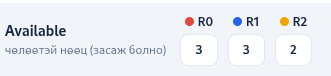
\includegraphics[width=.63\linewidth]{images/free.png}\\[4pt]

\includegraphics[width=.61\linewidth]{images/mode.png}
\captionof{figure}{Номын жишээ ачаалсны дараах хоёр хэсэг. Дээд зурагт сул нөөц, доод зурагт идэвхтэй Banker горим харагдана.}\label{fig:book}
\end{center}

\begin{minipage}[t]{.50\linewidth}\vspace{0pt}
\textbf{Зөвшөөрсөн хэрэгцээнээс хэтэрвэл.}
Номын анхны төлөв дээр P0-ийн R0 хэрэгцээ 7. Хүсэлтийн R0 нүдэнд 99 оруулахад эхний шалгалт дээр шалтгааныг «хүсэлт=99, Need=7» гэж харуулна. Энэ тохиолдолд цөм \code{error} хариу өгнө. Safety шалгалт, түр олголт хоёул алгасагдана.

Харин хүснэгт~\ref{tab:req}-ийн P4 хэрэгцээгээ хэтрүүлээгүй. Зөвхөн тухайн үеийн сул нэгж хүрээгүй тул \code{wait} гэсэн өөр шийдвэр гарсан.
\end{minipage}\hfill
\begin{minipage}[t]{.46\linewidth}\vspace{0pt}\centering
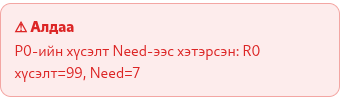
\includegraphics[width=\linewidth,height=72mm,keepaspectratio]{images/error.png}
\captionof{figure}[P0-ийн оролтын алдаа]{P0-ийн $(99,0,0)$ хүсэлтийг шалгасан нь.}\label{fig:err}
\end{minipage}
\newpage
\subsection{Нөөцийн граф ба үйлдлийн түүх}
Графын тойрог бүр процесс, хүрээтэй хайрцаг бүр нэг төрлийн нөөц. Хайрцаг доторх өнгөт цэг тухайн өнгийн процесст олгосон нэгжийг, цагаан цэг сул нэгжийг илэрхийлнэ. Зураг~\ref{fig:graph}-т R0-ийн 10-аас гурав, R1-ийн таваас гурав, R2-ын долоогоос хоёр нь сул байна. Энэ нь хүснэгтийн Available $(3,3,2)$-той таарна.
\fig{.85}{82mm}{graph}{Нөөцийн нэгж, хуваарилалтын сум ба дуусах дараалал}{fig:graph}

Цэнхэр сум нөөцөөс процесс руу чиглэж, одоо эзэмшиж буй Allocation-ийг заана. P1 дээрх жижиг дугуй доторх «1» нь эхэлж дуусах процессыг зааж байна. Процесс дээр хулгана аваачих буюу дарахад тухайн процессын Need сум тодорно. Олон процессын хэрэгцээг зэрэг харах бол «Need сумыг үргэлж харуулах» сонголтыг асаана. «Дараах» товчоор нэг алхам урагшлах бүрдээ Work-ийг хүснэгт~\ref{tab:safety}-ийн сүүлийн баганатай тулгаж болно.

\fig{1}{40mm}{history}{Хуудсыг шинэчлэхийн өмнөх хүсэлтийн тоолуур}{fig:log}
Зураг~\ref{fig:log}-т нэг хүсэлт аюултай гэж татгалзсан байна. Түүх нь Request ба Release үйлдэл бүрийг бичнэ. Дээрх дөрвөн тоолуур зөвхөн Request-ийн үр дүнг тоолдог. Хөтчөө шинэчлэхэд тухайн табын түүх, тоолуур тэглэгдэнэ. Сервер ажиллаж байгаа цагт өмнөх нөөцийн хуваарилалт хадгалагдах тул шинэчилсний дараа Available-ийг серверээс дахин уншина.
\newpage
\subsection{3×2 ба 10×5 жишээг харьцуулах нь}
\textbf{3 процесс, 2 нөөц.} Эхний Available $(1,1)$, P0, P1, P2-ын Need харгалзан $(2,2)$, $(2,1)$, $(3,2)$ байна. Бүгдэд R0-оос дор хаяж хоёр нэгж шаардагдах тул эхэлж дуусах процесс олдохгүй. «Нөөц чөлөөлөх» үйлдлийг сонгон P0-ийн эзэмшиж буй $(2,1)$-г буцаавал Available $(3,2)$ болно. Энэ үйлдэл P0-ийн Max-ийг өөрчлөхгүй учраас Allocation тэглэхэд өөрийнх нь Need $(4,3)$ болж өснө. Харин P1 одоо дуусаж чадна.

\tbl{3×2 жишээнд нөөц чөлөөлсний дараах дараалал}{tab:small}{
\begin{tabularx}{\linewidth}{YCCC}\toprule
\hd Дуусах процесс & \textbf{Work өмнө} & \textbf{Чөлөөлөх} & \textbf{Work дараа}\\\midrule
P1 & $(3,2)$ & $(1,2)$ & $(4,4)$\\
P0 & $(4,4)$ & $(0,0)$ & $(4,4)$\\
P2 & $(4,4)$ & $(2,0)$ & $(6,4)$\\\bottomrule
\end{tabularx}}
P0 дуусахад Work нэмэгдэхгүй байгаа нь зөв. Энэ процесс өмнөх Release үйлдлээр эзэмшиж байсан бүх нөөцөө аль хэдийн буцаасан. Бүх процесс дараалалд орсон тул төлөв SAFE болсон.

\textbf{10 процесс, 5 нөөц.} «Том туршилт 10×5» жишээнд эхний Work $(3,3,3,5,5)$ бөгөөд P0-оос P9 хүртэл дараалан дуусч чадна. Зураг~\ref{fig:big} дэх ногоон зурваст графын эхний Work болон дараалал харагдана. Жишээлбэл P0 дуусахад Work $(4,5,6,5,8)$ болно. Хоёр утгын зөрүү $(1,2,3,0,3)$ нь P0-оос чөлөөлөгдөх нөөц юм.
\fig{1}{58mm}{big}{10×5 жишээний эхний Work ба аюулгүй дараалал}{fig:big}
Эдгээр жишээний өгөгдлийг \code{src/ui/scenarios.json} файлаас вэб болон тест хоёулаа уншина. 3×2 жишээ нь Release-ийн дараа төлөв шилжихийг, 10×5 нь олон процесс, нөөцтэй үед аюулгүй дараалал бүх процессыг багтааж байгааг шалгадаг.
\newpage
